%%
% This is an Overleaf template for presentations
% using the TUM Corporate Desing https://www.tum.de/cd
%
% For further details on how to use the template, take a look at our
% GitLab repository and browse through our test documents
% https://gitlab.lrz.de/latex4ei/tum-templates.
%
% The tumbeamer class is based on the beamer class.
% If you need further customization please consult the beamer class guide
% https://ctan.org/pkg/beamer.
% Additional class options are passed down to the base class.
%
% If you encounter any bugs or undesired behaviour, please raise an issue
% in our GitLab repository
% https://gitlab.lrz.de/latex4ei/tum-templates/issues
% and provide a description and minimal working example of your problem.
%%

\documentclass{setbeamer}

\usepackage{scrextend}
\changefontsizes{8pt}

\usepackage{tikz}
\usetikzlibrary{calc}
\usetikzlibrary{positioning}

\usepackage{marvosym}

% https://tex.stackexchange.com/questions/196794/how-can-you-create-a-vertical-timeline
% Style and colors adjusted for TUM-Theme
\usepackage{xcolor}
% maybe vline after {$bullet$} for visual clarity, but this produced seams. I couldn't get rid of them...
\newcommand\ytl[2]{
\parbox[b]{8em}{\hfill{\color{TUMExtTeal}\bfseries\sffamily #1}~$\cdots\cdots$~}\,\makebox[0pt][c]{$\bullet$}\quad \parbox[c]{4.5cm}{\vspace{7pt}\color{TUMGrayDark}\raggedright\sffamily #2\\[7pt]}\\[-3pt]}

\newcommand{\myline}[3][TUMBlack]{
    \path(#2.south) --(#3.north)  coordinate[pos=0.4](mid);
    \ifthenelse{\equal{#1}{black}}
    {\draw[-latex, draw=#1] (#2.south) |- (mid) -| (#3.north);}
    {\draw[-latex, draw=#1, very thick] (#2.south) |- (mid) -| (#3.north);}
}

% presentation metadata
\title{Linux and Basic Tools}
\subtitle{Overview and Usage}

\institute{\theChairName\\\theDepartmentName\\\theUniversityName}
\date[\today]{\today}

\footline{\insertauthor~|~\insertshorttitle~|~\insertshortdate}

\begin{document}
 
\maketitle

\section{Linux}
% Linux ist hier noch unbekannt. Sagen dass linux ein bs ist wie windows und macos

% https://www.zdnet.com/article/minixs-creator-would-have-liked-knowing-intel-was-using-it
% https://de.wikipedia.org/wiki/Minix_(Betriebssystem)
% https://de.wikipedia.org/wiki/Linus_Torvalds
% https://de.wikipedia.org/wiki/Unix
% https://de.wikipedia.org/wiki/Geschichte_von_Linux
\begin{frame}{Linux}
    Linux is a generic name for a family of open-source Unix-like operating systems.\\

    \begin{itemize}
        \item Based on the Linux kernel (initially by Linus Torvalds in 1991)
        \item Large-scale free open source project
        \item Linux distribution includes, kernel, system software, libraries
        \item Popular distributions:  Debian, Fedora Linux, Arch Linux, Rocky Linux, and Ubuntu
        \item Commercial distributions: Red Hat Enterprise Linux, SUSE Linux Enterprise
        \item Originally developed for x86 architecture
    \end{itemize}
    \vspace{0.3cm}

	We use Linux on personal computers, edge devices (watch, cellphone\dots ), embedded systems (microwave, car\dots), servers, and high performance computing (HPC) systems.
\end{frame}



% Die Slide soll Überblick geben über die unterschiede, nicht im tiefsten detail alles erläutern
\begin{frame}{Linux Distributions}
    The distributions differ in 
    \begin{itemize}
        \item Package Manager and Installer
        \item Architecture (x86-64 for AMD and Intel, Apple, ARM\dots) % Apple shift von x86-64 auf 
        \item Hardware Support (i.e. drivers for non-standard hardware) % ungenau behandeln
        \item Release Cycle 
        \item Documentation % ARCH Wiki namen aufschreiben (allgemein verwendbar).
        \item Support % Ubuntuusers, Stack Exchange namen aufschreiben
        \item License
    \end{itemize}
    Overall, Ubuntu is probably a good choice for personal computers, for HPC systems, one typically relies on Rocky Linux, Red Hat Enterprise Linux, etc.
\end{frame}

\section{The File System}

% Entwickler der Filesysteme dynamisch per hand hinschreiben (Microsoft, Oracle, etc.)
\begin{frame}{File Systems}
    The file system organizes the data on the physical drives (HDD/SSD/USB, etc). There exist different formats to organize the data, and not all formats are compatible with all operating systems.
    \begin{itemize}
        \item Linux-typical:
        \begin{itemize}
            \item ext4
            \item Btrfs
        \end{itemize}
        \item Windows-typical:
        \begin{itemize}
            \item FAT32 % bsp wie groß 4gb sind. So typische DVD size, 4GB hinschreiben
            \item exFAT
            \item NTFS
        \end{itemize}
        \item MacOS-typical:
        \begin{itemize}
            \item APFS
            \item HFS+
        \end{itemize}
    \end{itemize}
    FAT32 is supported also by MacOS and Linux, ext4 requires additional drivers on Windows and MacOS.
\end{frame}

% Ich bin mir unsicher über das layout der Slide
% Die gemischte nutzung von mintinline und TUMCodeInline ist tatsächlich bewusst
% Vielleicht hier schon auf hidden files eingehen (Unix hidden files mit .)
\begin{frame}{Directories and file names}
	File systems typically support organizing files into \textbf{directories}, also called \textbf{folders}, which segregate files into groups. \\


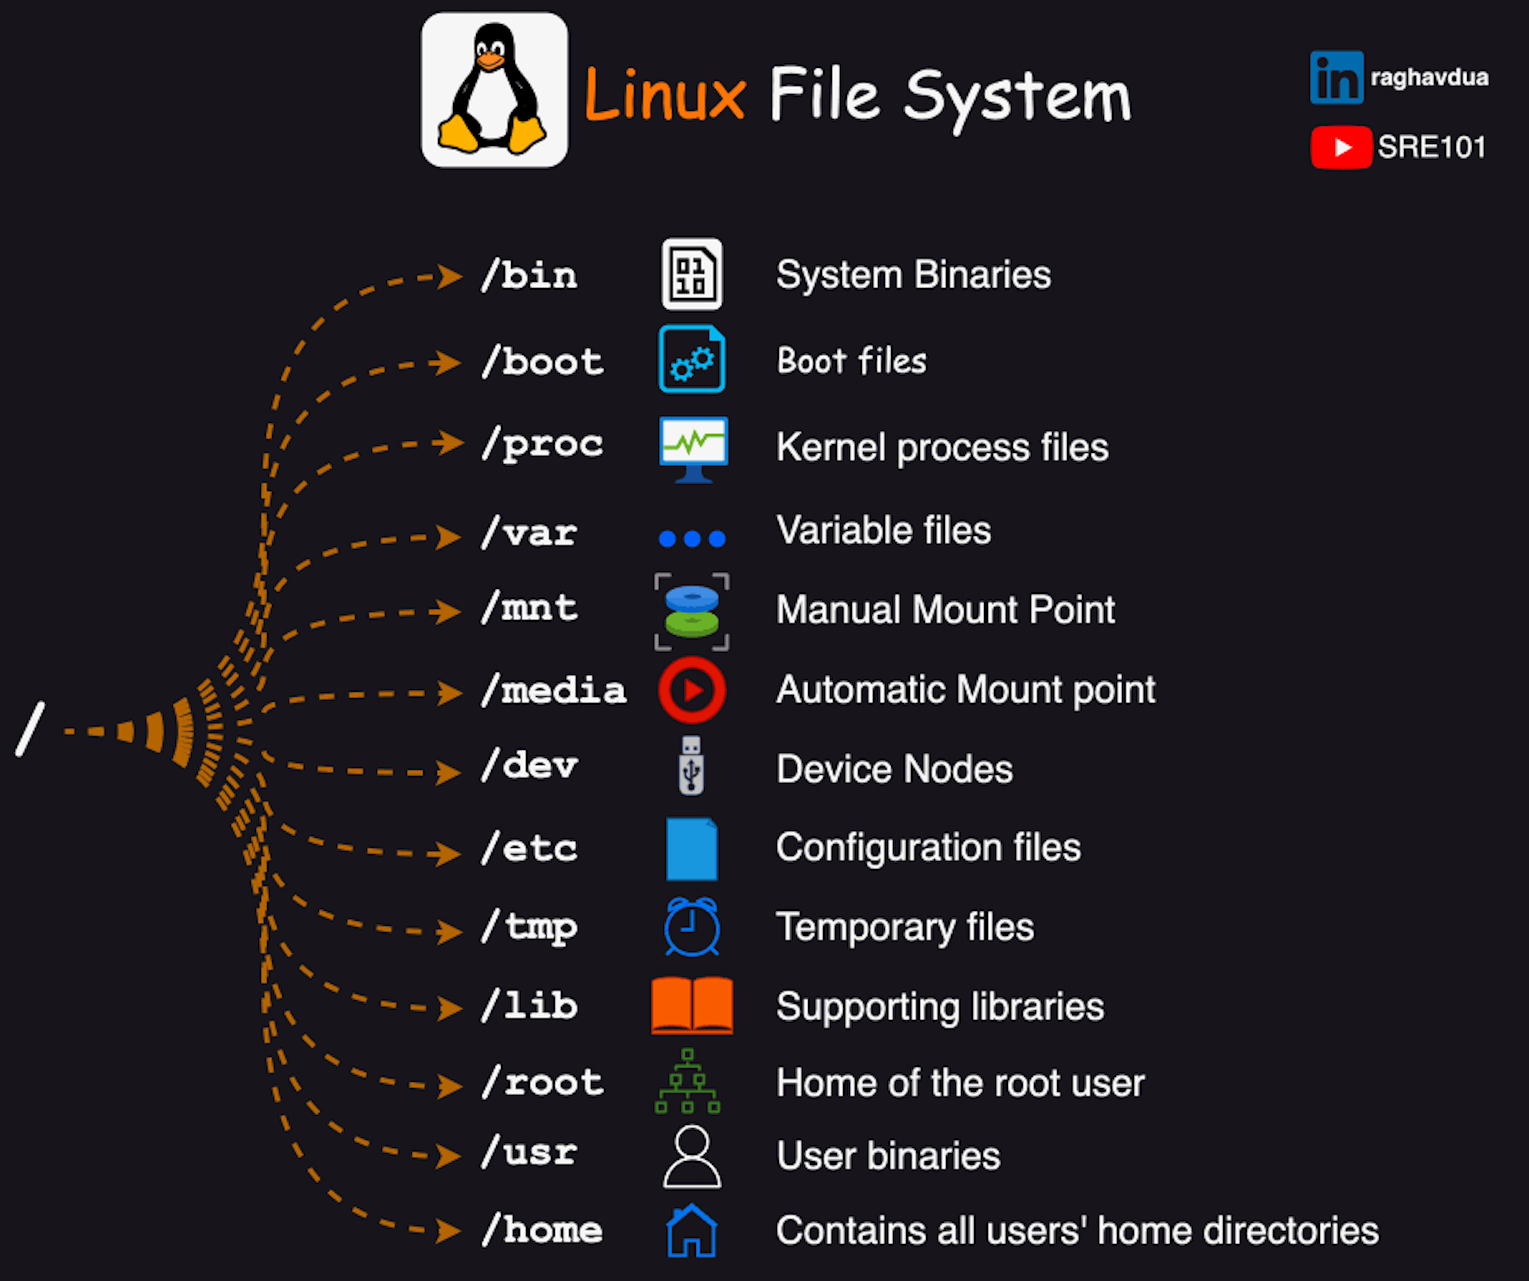
\includegraphics[width=.5\columnwidth]{resources/folders.png}


\end{frame}



% Ich bin mir unsicher über das layout der Slide
% Die gemischte nutzung von mintinline und TUMCodeInline ist tatsächlich bewusst
% Vielleicht hier schon auf hidden files eingehen (Unix hidden files mit .)
\begin{frame}{Directories and file names}
	File systems typically support organizing files into \textbf{directories}, also called \textbf{folders}, which segregate files into groups. \\
	
A \textbf{file name}, or \textbf{filename}, identifies a file for an application or user. For this, a file name has to be unique in a folder. \\

The \textbf{path} is the global address of a file.\\


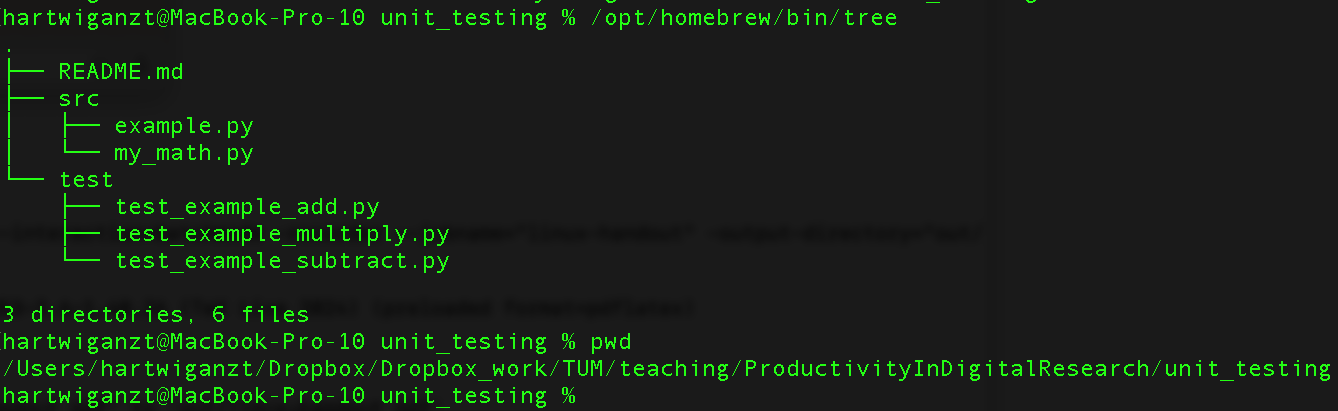
\includegraphics[width=.95\columnwidth]{resources/folder_filenames.png}


\end{frame}



\begin{frame}{Navigating and organizing the file system}
    \begin{itemize}
        \item \TUMCodeInline{text}{ls} show content of current folder
        \item \TUMCodeInline{text}{ls -l} show content of current folder with details
        \item \TUMCodeInline{text}{cd ..} go up one folder
        \item \TUMCodeInline{text}{cd foo} go into folder ``foo''
        \item \TUMCodeInline{text}{pwd} show path to current folder
        \item \TUMCodeInline{text}{mkdir foo} create folder ``foo''
        \item \TUMCodeInline{text}{cp (-r) foo bar} copy ``foo'' to ``bar'' (-r copies all content)
        \item \TUMCodeInline{text}{mv foo bar} rename ``foo'' to ``bar''
        \item \TUMCodeInline{text}{rm (-r) bar} remove ``bar'' 
        % \item \TUMCodeInline{text}{{chmod u+x foo.sh} make skript ``foo.sh'' executable 
    \end{itemize}
\end{frame}



\section{Terminal use}

\begin{frame}{The Terminal}
    The terminal is an interface for the user to interact with the computer. (In the past, before GUIs were supported, it was the only form of interaction).

    \vspace{0.3cm}

    The terminal
    \begin{itemize}
        \item accepts commands from the user
        \item displays output from the computer
        \item allows for full control of all computer applications
    \end{itemize}
\end{frame}

\begin{frame}{What are the advantages of the terminal?}
    \begin{itemize}
        \item Interaction is efficient and precise
        \item Allows for automation (scripts)
        \item Flexibility in the usage of programs and interaction between
        \item Resource efficient:
        \begin{itemize}
            \item Remote connection requires little bandwidth
            \item Remote connection via terminal usually possible
            \item Terminal use is very similar across operating systems
        \end{itemize}
        \item Servers usually do not support GUI
    \end{itemize}
\end{frame}




% https://unix.stackexchange.com/questions/285575/whats-the-difference-between-a-flag-an-option-and-an-argument
\begin{frame}[fragile]{Command Line Arguments}
    \begin{TUMCodeBlock}{Command Arguments and Options}{text}
        command [OPTION...] arguments
    \end{TUMCodeBlock}

    \vspace{0.3cm}

    \begin{itemize}
        \item \TUMCodeInline{text}{command}\textemdash The command to be executed

        \item \TUMCodeInline{text}{[OPTION...]}\textemdash Options for the command
        \begin{itemize}
            \item \emph{Long-options} (e.g. \TUMCodeInline{text}{--version}) and \emph{Short-options} (e.g. \TUMCodeInline{text}{-v})
            \item Some \emph{options} take additional arguments
            \item \emph{Options} without \emph{arguments} are called \emph{flags}
            \item Useful \emph{flags}: \TUMCodeInline{text}{--help} (or \TUMCodeInline{text}{-h}) and \TUMCodeInline{text}{--version} (or \TUMCodeInline{text}{-v})
        \end{itemize}

        \item \TUMCodeInline{text}{arguments}\textemdash Additional arguments (e.g. files, paths, etc.)
    \end{itemize}

   
\end{frame}


%check 1 


% man, ls, cd, rm, mkdir, touch, cat, sudo, echo
% die reichen für eine basic benutzung der kommandozeile und vermutlich für das erste Aufgabenblatt
\begin{frame}{Essential Commands}
    % TAR XKCD
    \begin{figure}[h]
        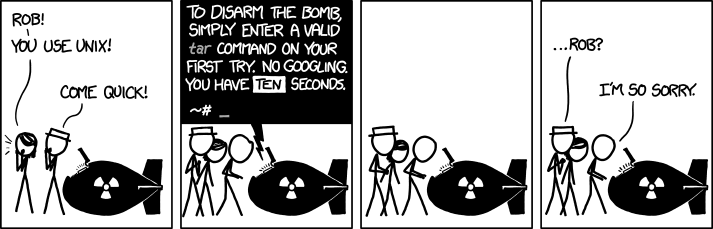
\includegraphics[width=14.5cm, keepaspectratio]{./resources/tar.png}
        \caption*{\myhref{https://xkcd.com/1168/}{xkcd 1168}}
    \end{figure}

    % tar command beispiel, den joke erklären (so doof es auch ist):
    % tar -cvzf archive.tar *

    \pause
    \centering
    You do not need to know all commands by heart, but it is useful!
\end{frame}

\begin{frame}{Basic Commands | \texttt{man}}
    Stands for ``manual''.

    \vspace{0.3cm}

    Opens the usage description for a program.

    \vspace{0.3cm}

    \begin{itemize}
        \item \TUMCodeInline{text}{man <command>} (e.g., \TUMCodeInline{sh}{man man})
    \end{itemize}
\end{frame}

\begin{frame}{Basic Commands | \texttt{ls}}
    Stands for ``list''.

    \vspace{0.3cm}

    Lists the content of a folder.

    \vspace{0.3cm}

    Usage:
    \begin{itemize}
        \item \TUMCodeInline{text}{ls}
        \item \TUMCodeInline{text}{ls path/to/folder}
        \item \TUMCodeInline{text}{ls -a}\textemdash Shows also hidden files (folders/files that start with \TUMCodeInline{sh}{.} )
        \item \TUMCodeInline{text}{ls -l}\textemdash Lists details  (type, size, access rights, date\dots)
    \end{itemize}
\end{frame}

\begin{frame}{Essential Commands | \texttt{cd}}
    Stands for ``change directory''.

    \vspace{0.3cm}

    Change of the \emph{current working directory}.

    \vspace{0.3cm}

    Usage:
    \begin{itemize}
        \item \TUMCodeInline{text}{cd path/to/folder}
        \item \TUMCodeInline{text}{cd ..}\textemdash Change to the parent directory
        \item \TUMCodeInline{text}{cd ~}\textemdash Change to the \emph{Home} directory
    \end{itemize}
\end{frame}

\begin{frame}{Basic Commands | \texttt{pwd}}
    Stands for ``print working directory''.

    \vspace{0.3cm}

    Shows the \emph{current working directory}.

    \vspace{0.3cm}

    Usage:
    \begin{itemize}
        \item \TUMCodeInline{text}{pwd}
    \end{itemize}
\end{frame}

\begin{frame}{Basic Commands | \texttt{cat}}
    Stands for ``concatenate files and print''.

    \vspace{0.3cm}

    Displays files.

    \vspace{0.3cm}

    Usage:
    \begin{itemize}
        \item \TUMCodeInline{text}{cat test.txt}\textemdash Prints the content of \TUMCodeInline{text}{test.txt}
        \item \TUMCodeInline{text}{cat one.txt two.txt}\textemdash Prints the content of \TUMCodeInline{text}{one.txt} and \TUMCodeInline{text}{two.txt}
    \end{itemize}
\end{frame}

\begin{frame}{Basic Commands | \texttt{echo}}
    Gibt den Angegebenen Text wieder aus.

    \vspace{0.3cm}

    Usage:
    \begin{itemize}
        \item \TUMCodeInline{text}{echo "some text"}
    \end{itemize}
\end{frame}

\begin{frame}{Basic Commands | \texttt{mkdir}}
    Stands for ``make directory''.

    \vspace{0.3cm}

    Creates folder.

    \vspace{0.3cm}

    Usage:
    \begin{itemize}
        \item \TUMCodeInline{text}{mkdir folder}\textemdash creates folder \TUMCodeInline{text}{folder} in current directory
        \item \TUMCodeInline{text}{mkdir f1 f2 f3}\textemdash creates folders \TUMCodeInline{text}{f1}, \TUMCodeInline{text}{f2} and \TUMCodeInline{text}{f3} in current directory
    \end{itemize}
\end{frame}

\begin{frame}{Basic Commands | \texttt{rm}}
    Stands for ``remove''.

    \vspace{0.3cm}

    Removes files or folders

    \vspace{0.3cm}

    Usage:
    \begin{itemize}
        \item \TUMCodeInline{text}{rm test.txt}
        \item \TUMCodeInline{text}{rm -d empty-folder}
        \item \TUMCodeInline{text}{rm -r nonempty-folder}\textemdash Folder with content have to be deleted recursively
        \item \TUMCodeInline{text}{rm -f test.txt}\textemdash Forces the deletion
    \end{itemize}
\end{frame}


\begin{frame}{Basic Commands | \texttt{mv}}
    Stands for ``move''.

    \vspace{0.3cm}

    Change a file location or renames a folder.

    \vspace{0.3cm}

    Usage:
    \begin{itemize}
        \item \TUMCodeInline{text}{mv path/to/file new/path/}\textemdash Moves \TUMCodeInline{text}{file} from \TUMCodeInline{text}{path/to/} to \TUMCodeInline{text}{new/path/}
        \item \TUMCodeInline{text}{mv path/to/file new/path/elif}\textemdash Changes the location and the filename from \TUMCodeInline{text}{file} to \TUMCodeInline{text}{elif} 
    \end{itemize}
\end{frame}

\begin{frame}{Basic Commands | \texttt{cp}}
    Stands for ``copy''.

    \vspace{0.3cm}

   Copies files or folders.

    \vspace{0.3cm}

    Usage:
    \begin{itemize}
        \item \TUMCodeInline{text}{cp path/to/file other-path/to/copy}\textemdash Copies \TUMCodeInline{text}{file} from \TUMCodeInline{text}{path/to/} to \TUMCodeInline{text}{other-path/to/} and stores the copy as \TUMCodeInline{text}{copy}
    \end{itemize}
\end{frame}

% https://www.techtarget.com/searchsecurity/definition/sudo-superuser-do
\begin{frame}{Basic Commands | \texttt{sudo}}
    Stands for ``su-do'' (``substitute user do'', or ``superuser do'').

    \vspace{0.3cm}

    Call a command as a different user (usually the \emph{superuser's}).

    \vspace{0.3cm}

    \TUMCodeInline{text}{sudo} is needed if the user rights of the current user are not sufficient:
    \begin{itemize}
        \item \TUMCodeInline{text}{sudo dnf install terminator}\textemdash the installation of a new package (``terminator'') requires the rights of a \emph{superuser}
    \end{itemize}
\end{frame}

% https://www.w3resource.com/linux-system-administration/control-operators.php
\begin{frame}[fragile]{Control Operators}
    \TUMCodeInline{text}{&&}
    \begin{itemize}
        \item Combine two commands -- the second command is only executed if the first was successful.
        \item For example: \TUMCodeInline{text}{cd foo && ls}
    \end{itemize}

    \vspace{0.3cm}

    \TUMCodeInline{text}{||}
    \begin{itemize}
        \item Combine two commands -- the second command is only executed if the first was \textbf{not} successful.
        \item For example: \TUMCodeInline{text}{cd foo || echo "Folder does not exist"}
    \end{itemize}

    \vspace{0.3cm}

    \TUMCodeInline{text}{;}
    \begin{itemize}
        \item Combine two commands.
        \item For example: \TUMCodeInline{text}{cd folder; ls}
    \end{itemize}
\end{frame}

\begin{frame}{Control Operators}
    \TUMCodeInline{text}{&}
    \begin{itemize}
        \item The precious command is executed in the background
        \item For example: \TUMCodeInline{text}{sleep 10 &}
    \end{itemize}

    \vspace{0.3cm}

    \TUMCodeInline{text}{>} and \TUMCodeInline{text}{>>}
    \begin{itemize}
        \item Redirects the output, \TUMCodeInline{text}{>} overwrites previous content.
        \item For example: \TUMCodeInline{text}{echo "HelloWorld!" > greeting.txt} or \TUMCodeInline{text}{echo "HelloWorld!" >> greeting.txt}
    \end{itemize}

    \vspace{0.3cm}

    \TUMCodeInline{text}{|} (called ``Pipe'')
    \begin{itemize}
        \item The output of the precious command is the input of the next command
        % zuerst einmal fortune ausführen und dann einmal cowsay
        \item For example: \TUMCodeInline{text}{ls | sort}
    \end{itemize}
\end{frame} 



\begin{frame}{Useful Tricks}
   
    \begin{itemize}
        \item Recall previous command: upward arrow
        \item Complete path: tab
        \item Delete current input: Ctrl + u
        \item Cancel current input: Ctrl + c
        \item Copy terminal input: Ctrl + Shift + c
        \item Copy terminal input: Ctrl + Shift + v
        \item Remove recent command + output: Ctrl + l
    \end{itemize}
    
\end{frame} 




\section{Access Control}

\begin{frame}{Access Control}
    Controlling the access and privileges of users is important!
    
    \begin{itemize}
        \item Data can be private, sensitive, export control\dots
        \item Often, many users interact with the same file system
    \end{itemize}

    \pause
    \vspace{0.3cm}

       Linux uses \emph{Access-Control-List} (\emph{ACL}\,)
    \begin{itemize}
        \item \emph{ACL} is operating from the object size {\Large \MVRightarrow} Every object exposes different rights for different groups
        \item Rights given to \emph{Owner}, \emph{Group} and \emph{Other}
        \item Rights include:
        \begin{itemize}
            \item \textbf{R}ead 
            \item \textbf{W}rite
            \item e\textbf{X}ecute
        \end{itemize}
    \end{itemize}

    \pause
    \vspace{-1.5cm}
    \hspace{5cm}
	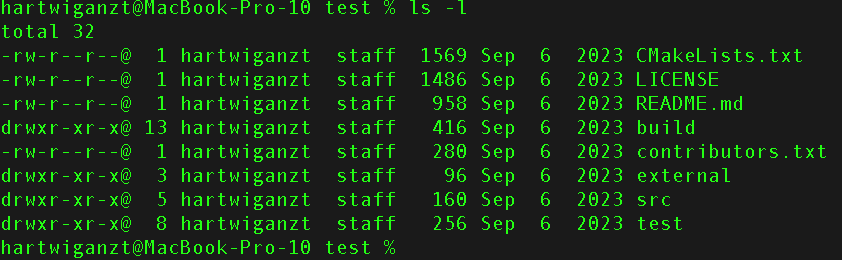
\includegraphics[width=.6\columnwidth]{resources/ls-l.png}

\end{frame}


\begin{frame}{Access Control}

To change the permissions of a file, one uses the \TUMCodeInline{text}{chmod} command, with the following syntax:
\begin{itemize}


\item
\TUMCodeInline{text}{chmod [references][operator][modes] filename}
The references are shorthand (\TUMCodeInline{text}{u}, \TUMCodeInline{text}{g}, or \TUMCodeInline{text}{o}) for each class. The operator determines whether to add (+), remove (-) or explicitly set (=) the particular permissions. The modes are read \TUMCodeInline{text}{(r)}, write \TUMCodeInline{text}{(w)}, or execute \TUMCodeInline{text}{(x)}.
\item
For example, to add the execute permission for the \TUMCodeInline{text}{user} to \TUMCodeInline{text}{file1}:\\
\TUMCodeInline{text}{chmod u+x file1}
\item
To remove the write permission for \TUMCodeInline{text}{others} for \TUMCodeInline{text}{file2}:

\TUMCodeInline{text}{chmod o-w file2}
\item
You can combine multiple references and modes to set the desired access all at once. For example, to explicitly make \TUMCodeInline{text}{file3} readable and executable to everyone:\\

\TUMCodeInline{text}{chmod ugo=rx file3}
\item
The all \TUMCodeInline{text}{(a)} mode is the same as \TUMCodeInline{text}{ugo}, allowing the previous command to be expressed as:

\TUMCodeInline{text}{chmod a=rx file3}
\end{itemize}
For more information on changing permissions, run \TUMCodeInline{text}{man chmod}

\end{frame}



\section{Environment Variables}

\begin{frame}{Environment Variables}
    \emph{Environment Variables} enable passing configurable variables to processes via the environment.

    \vspace{0.3cm}

    Beispiele für \emph{Environment Variables}:
    \begin{itemize}
        \item HOSTTYPE\textemdash Architecture of the computer (e.g. \emph{x86-64})
        \item HOME\textemdash Path to \TUMCodeInline{sh}{/home/<username>}
        \item PWD\textemdash Path to current working directory''
        \item PATH\textemdash Path to executables
        \item TEMP/TMP\textemdash Path to temporary data
    \end{itemize}

    % Nicht wirklich necessary, kann man einfach sagen
    %\vspace{0.3cm}
    %Alle Prozesse auf einem Unixoidem Betriebssystem oder Windows erhalten einen eigenen separaten Satz an \emph{Environment Variables} die bei der Erstellung des Prozesses erstellt werden.
\end{frame}

\section{SSH}

%https://wiki.ito.cit.tum.de/bin/view/Informatik/Helpdesk/Ssh/#H1.1.SSHVerbindungmitPasswort
\begin{frame}[fragile]{SSH}
    SSH stands for \emph{Secure Shell}:
    \begin{itemize}
        \item Enables a secure connection between servers (e.g. Internet)
        \item Enables secure remote server administration
        \item Identities, passwords, files are encrypted
    \end{itemize}

    \pause
    \vspace{0.3cm}

    We can connect to a remote server this way:

    \vspace{0.3cm}

    \begin{TUMCodeBlock}{}{sh}
        ssh <username>@lxhalle.in.tum.de
    \end{TUMCodeBlock}
    {\Large \MVRightarrow} Connection can be closed with \TUMCodeInline{text}{exit}.

    \vspace{0.3cm}

    % Needed to escape # in URL
    In the first connection, the fingerprint \myhref{https://wiki.ito.cit.tum.de/bin/view/Informatik/Helpdesk/Ssh/\#H0.Fingerprints}{Fingerprints} need to be verified. (Is it the right server?)
\end{frame}

% https://www.bsi.bund.de/SharedDocs/Downloads/EN/BSI/Publications/TechGuidelines/TG02102/BSI-TR-02102-1.pdf?__blob=publicationFile
% Federal Office for Information Security (as of Jan 2023)
\begin{frame}{SSH Keys}
    Instead of verification with a password, we can also use a set of ssh keys. \myhref{https://wiki.ito.cit.tum.de/bin/view/Informatik/Helpdesk/Ssh/\#H1.3.SSHKey}{Generation}:
    \begin{itemize}
        % Increased bit depth for RSA Key for compliance with current standards
        \item \TUMCodeInline{sh}{ssh-keygen -t rsa -b 4096} for an \emph{RSA} (Rivest-Shamir-Adleman) key pair
        \item \TUMCodeInline{sh}{ssh-keygen -t ed25519} for an \emph{ECC} (Elliptic Curve Cryptography) key pair
    \end{itemize}

    \vspace{0.3cm}

    A key pair consists of:
    \begin{itemize}
        \item a public key (e.g. \TUMCodeInline{sh}{~/.shh/id_ed25519.pub})
        \item a private key (e.g. \TUMCodeInline{sh}{~/.ssh/id_ed25519})
    \end{itemize}
    {\Large \MVRightarrow} It is an asymmetric encryption strategy!

    \vspace{0.3cm}

    \begin{itemize}
        % Hier erwähnen, dass in den späteren vcs Slides noch genauer darauf eingegangen wird
        \item The public key can be given to anyone. I.e. stored on the server we want to access. (\myhref{https://wiki.ito.cit.tum.de/bin/view/Informatik/Helpdesk/Ssh}{Rechnerhalle}, \myhref{https://doku.lrz.de/ssh-tutorial-10746941.html}{LRZ}, \myhref{https://docs.github.com/en/authentication/connecting-to-github-with-ssh}{GitHub}, etc.)
        \item \textbf{The private key has to be kept private! Never share it!}
    \end{itemize}
\end{frame}

% Hier muss man vorsichtig sein. Die eigentliche SSH Verbindung ist symmetrisch verschlüsselt (AES). Aufpassen, dass durch die Folien nicht etwas falsches suggeriert wird. Eine Sinnvolle Waage finden zwischen dem was im Vorkurs für ein basic Verständnis wichtig ist und dem was in der Realität passiert. Anwendungsbezug prüfen und im Zweifel den "Content Scope" reduzieren.
%\begin{frame}{Asymmetrische Verschlüsselung}
    % Ich glaub ich yeete diese Slide. Sie ist nicht strictly necessary
%\end{frame}



\section{Code Editing}

\begin{frame}{Editors}
    % TAR XKCD
    \begin{figure}[h]
        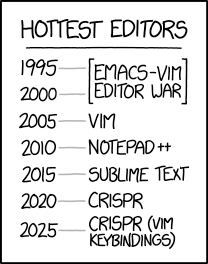
\includegraphics[width=4.5cm, keepaspectratio]{./resources/hottest_editors.png}
        \caption*{\myhref{https://xkcd.com/1823/}{xkcd 1823}}
    \end{figure}

    % auch hier den joke wieder ein bissel erklären (ist doof, aber eh...)
    % Letztendendes will ich mit dem xkcd sagen, dass die Unterscheidung Text Editor und Code Editor beschissen ist.
    % Im Internet findet man dazu nur wild unterschiedliche Definitionen die nicht miteinander kompatibel sind.
    % Der xkcd fasst das super zusammen weil dieser 'Editoren' noch allgemeiner sieht. Weswegen 'crispr' gelistet wird (GEN-Editor)
\end{frame}

\begin{frame}{Text Editors and IDE's}
    \emph{Text editors} are lightweight tools for editing text or coding:
    \begin{itemize}
        \item nano
        \item vi, \myhref{https://www.vim.org/}{vim}, \myhref{https://neovim.io}{neovim}
        \item \myhref{https://www.sublimetext.com}{Sublime Text}
        \item \myhref{https://code.visualstudio.com}{Visual Studio Code}
        % "freiere" Version von VS Code ohne Telemetrie von Microsoft
        \item \myhref{https://vscodium.com}{VSCodium}
    \end{itemize}

    \pause
    \vspace{0.3cm}

    \emph{IDE} Stands for \emph{Integrated Development Environment}. \emph{IDE's} add tools that ease the software development:
    \begin{itemize}
        \item \myhref{https://www.jetbrains.com/de-de/idea}{IntelliJ}
        \item \myhref{https://www.eclipse.org/downloads}{Eclipse}
        \item \myhref{https://visualstudio.microsoft.com/de}{Visual Studio}
    \end{itemize}
\end{frame}

\begin{frame}{Terminal Editors}
    % immer available
    Terminal editors line \emph{nano}, \emph{vi}, \emph{vim} are pre-installed on almost every system.

    \pause
    \vspace{0.3cm}

    \textbf{nano}:
    \begin{itemize}
        \item Easy to use
        \item In the manual of nano, \TUMCodeInline{text}{^} refers to \emph{Ctrl}
        \item nano is quit with \TUMCodeInline{text}{^X} (\emph{Strg+X}\,) 
    \end{itemize}
\end{frame}

\begin{frame}{Terminal Editors}
    % vi zu vim. in vi keine text objects und konfiguration ist non existent. es gibt nur vanilla insert und normal mode
    % vim hat text object systeme, autocomplete, vimscript, packages plugins, searches, mehr settings wie incremental search, extended normal mode
    % neovim kann lua weil vimscript shit ist, nativer lsp, vim api in lua übersetzt

    \textbf{vim}:
    \begin{itemize}
        \item Operates with ``Modes'' (e.g. \textbf{INSERT-MODE} and \textbf{NORMAL-MODE})
        \item \emph{vim} starts in \textbf{NORMAL-MODE}, which allows the commands:
            \begin{itemize}
                \item \TUMCodeInline{text}{:q}\textemdash ``Quit'' (quits vim)
                \item \TUMCodeInline{text}{:w}\textemdash ``Write'' (writes the edited text)
                \item \TUMCodeInline{text}{:wq}\textemdash ``Write and Quit''
                \item \TUMCodeInline{text}{!} forces the command
                \item with \TUMCodeInline{text}{i} the editor changes to \textbf{INSERT-MODE}
            \end{itemize}
        \item The \textbf{INSERT-MODE} allows to
            \begin{itemize}
            	\item insert text
                \item change to \textbf{NORMAL-MODE} with \emph{ESC} 
            \end{itemize}
    \end{itemize}
\end{frame}

\section{Useful Commands}
% hier ist dann der ganze rest der commands (htop, grep, less, etc.)
% Die Slides über die commands kann man rauskopieren und dann in ein cheatsheet packen

\begin{frame}{Useful Commands | \texttt{grep}}
    Stands for ``\textbf{g}lobal \textbf{r}egular \textbf{e}xpression search and \textbf{p}rint''.

    \vspace{0.3cm}

    With \texttt{grep} we can search for patterns.
    \vspace{0.3cm}

    % 1973 veröffentlicht und Entwickelt von Ken Thompson
    % Ken nutzte das Programm bereits privat
    % Sein Abteilungsleiter Doug McIlroy (wusste noch nichts von grep) schlug Thompson ein solches Programm vor!
    % Thompson sagte dass er in der Nacht drüber nachdenken wird (nutzte die Zeit aber um Bugs zu fixen und letzte Verbesserungen zu machen) --> Daher auch die misconception, dass grep in einer Nacht geschrieben wurde.

    Usage:
    \begin{itemize}
        \item General use: \TUMCodeInline{text}{grep "RegEx" Datei-Muster}
        \item \TUMCodeInline{text}{grep "test" *.txt}\textemdash Returns the rows of the \TUMCodeInline{text}{.txt} files that contain \emph{test}
        \item \TUMCodeInline{text}{cat *.txt | grep "test"}\textemdash Often used in combination with pipes \TUMCodeInline{text}{|}
        \item Useful options are \TUMCodeInline{text}{-c} (for ``count'') and \TUMCodeInline{text}{-i} {for ``ignore-case''}
    \end{itemize}

    % Options wie -c (count) und -i (ignore-case)
\end{frame}

\begin{frame}{Useful Commands | \texttt{wc}}
    Stands for ``word count''.

    \vspace{0.3cm}
    
    Returns the number of rows, words, and bytes of a file.

    \vspace{0.3cm}

    Usage:
    \begin{itemize}
        \item \TUMCodeInline{text}{wc test.txt}
    \end{itemize}
\end{frame}

\begin{frame}{Useful Commands | \texttt{ping}}
    Sends an \emph{ICMP ECHO\_REQUEST} to the \emph{IP address} or \emph{URL}.

    \vspace{0.3cm}

   Useful to check the reachability of a website or server.

    \vspace{0.3cm}

    Usage:
    \begin{itemize}
        \item \TUMCodeInline{text}{ping zulip.in.tum.de}
    \end{itemize}
\end{frame}

\begin{frame}{Useful Commands | \texttt{scp}}
    Stands for ``\emph{OpenSSH} secure file copy''

    \vspace{0.3cm}

   Copies files over the network between servers

    \vspace{0.3cm}

    Usage:
    \begin{itemize}
        \item \TUMCodeInline{text}{scp path/to/local/file <username>@<remote-URL>:path/to/remote/copy}
        \item e.g. \TUMCodeInline{text}{scp test.txt <username>@lxhalle.in.tum.de:~/}
    \end{itemize}
\end{frame}

\begin{frame}{Useful Commands | \texttt{htop}}
    ``Task manager'' of Linux.

    \vspace{0.3cm}

    Usage:
    \begin{itemize}
        \item \TUMCodeInline{text}{htop}
    \end{itemize}
\end{frame}

\begin{frame}{Useful Commands | \texttt{who}}
    Shows who is logged in on a server.

    \vspace{0.3cm}

    Usage:
    \begin{itemize}
        \item \TUMCodeInline{text}{who}
    \end{itemize}
\end{frame}

\begin{frame}{Useful Commands | \texttt{more}}
   The content of a file is shown page-by-page.

    \vspace{0.3cm}

    Usage:
    \begin{itemize}
        \item \TUMCodeInline{text}{cat huge-file | more}
        \item \TUMCodeInline{text}{more huge-file}
    \end{itemize}
\end{frame}

\begin{frame}{Useful Commands | \texttt{less}}
    \texttt{less} similar to \texttt{more}, but more powerful.
    \begin{itemize}
        \item \texttt{less} does not have to process the whole file {\Large \MVRightarrow} faster
        \item allows for scrolling the file row by row
    \end{itemize}

    \vspace{0.3cm}

    Usage:
    \begin{itemize}
        \item \TUMCodeInline{text}{cat huge-file | less}
        \item \TUMCodeInline{text}{less huge-file}
    \end{itemize}
\end{frame}

\begin{frame}{Useful Commands | \texttt{alias}}
    Creates a alias command, a redirect.

    \vspace{0.3cm}

    Example:
    \begin{itemize}
        \item \TUMCodeInline{text}{alias wisdom="fortune | cowsay"}\textemdash allows to call the combined command in one command: \TUMCodeInline{text}{wisdom} instead of \TUMCodeInline{text}{fortune | cowsay}
    \end{itemize}

    \vspace{0.3cm}
    Only valid for the current session
    {\Large \MVRightarrow} A persistent alias can be created in the user environment (e.g. \TUMCodeInline{text}{~/.bashrc} or \TUMCodeInline{text}{~/.zshrc})
\end{frame}

\begin{frame}{Useful Commands | \texttt{history}}
    Displays the history of the used commands.

    \vspace{0.3cm}

    Usage:
    \begin{itemize}
        \item \TUMCodeInline{text}{history}
    \end{itemize}
\end{frame}

\begin{frame}{Useful Commands | \texttt{tree}}
    Displays the file system below the current path.

    \vspace{0.3cm}

    Usage:
    \begin{itemize}
        \item \TUMCodeInline{text}{tree}
    \end{itemize}
\end{frame}

\begin{frame}{Useful Commands | \texttt{pushd} and \texttt{popd}}
    Stands for ``push directory'' and ``pop directory''.

    \vspace{0.3cm}

    Simplifies to copy file paths.

    \vspace{0.3cm}

    Usage:
    \begin{enumerate}
        \item \TUMCodeInline{text}{pushd /bin}\textemdash stores \emph{pwd} and switches to \TUMCodeInline{text}{/bin}
        \item \TUMCodeInline{text}{popd}\textemdash switches \emph{pwd} to the previous path
    \end{enumerate}
\end{frame}


\end{document}
